\newpage
\section{Metodologia Experimental}

\subsection{Materiais}
O material utilizado foi:

\begin{itemize}
	\item Protótipo do conversor Boost disponível no laboratório.
	\item CI 4050.
	\item Resistor de 10K $\Omega$.
	\item Fonte de alimentação.
	\item Osciloscópio.
	\item Multímetro.
	\item Resistor variável de potência (50 $\Omega$).
\end{itemize}

Para execução do experimento, faz-se necessário executar os seguintes passos:

\begin{enumerate}
	\item montar o circuito gerador de onda quadrada conforme a figura \ref{f_gera_onda}, alimentando o CI com 12V;
	\item ajustar o gerador de funções para 100KHz, com razão cíclica abaixo de 50 \%;
	\item conectar os multímetros à placa do conversor boost como mostrado na figura \ref{f_buck};
	\item ajustar a tensão de entrada para 20V;
	\item variar a carga de modo a incrementar à corrente de saída em 500mA, mantendo a tensão de saída fixa em 30V;
	\item anotar o valor da tensão de entrada e saída e da corrente de entrada e saída;
	\item repetir os passos 5 e 6 até que a corrente de saída seja 3A ;
	\item ajustar a tensão de saída para 40V e repetir os passos 5,6 e 7;
	\item calcular o rendimento e o ganho estático;
	\item responder as perguntas:
	\begin{itemize}
		\item O ganho estático verificado na prática está de acordo com a teoria?
		\item Por que houve pequenas variações na razão cíclica para variações de carga?
		\item Traçar as curvas de rendimentos dos dois casos.
	\end{itemize}
\end{enumerate}

\begin{figure}[H]
	\centering
	\caption{Gerador de onda quadrada.}
	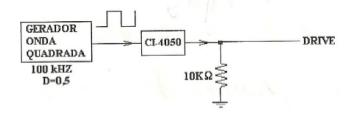
\includegraphics[scale=0.8]{gera_onda}
	\label{f_gera_onda}
\end{figure}

\begin{figure}[H]
	\centering
	\caption{Montagem do conversor Boost.}
	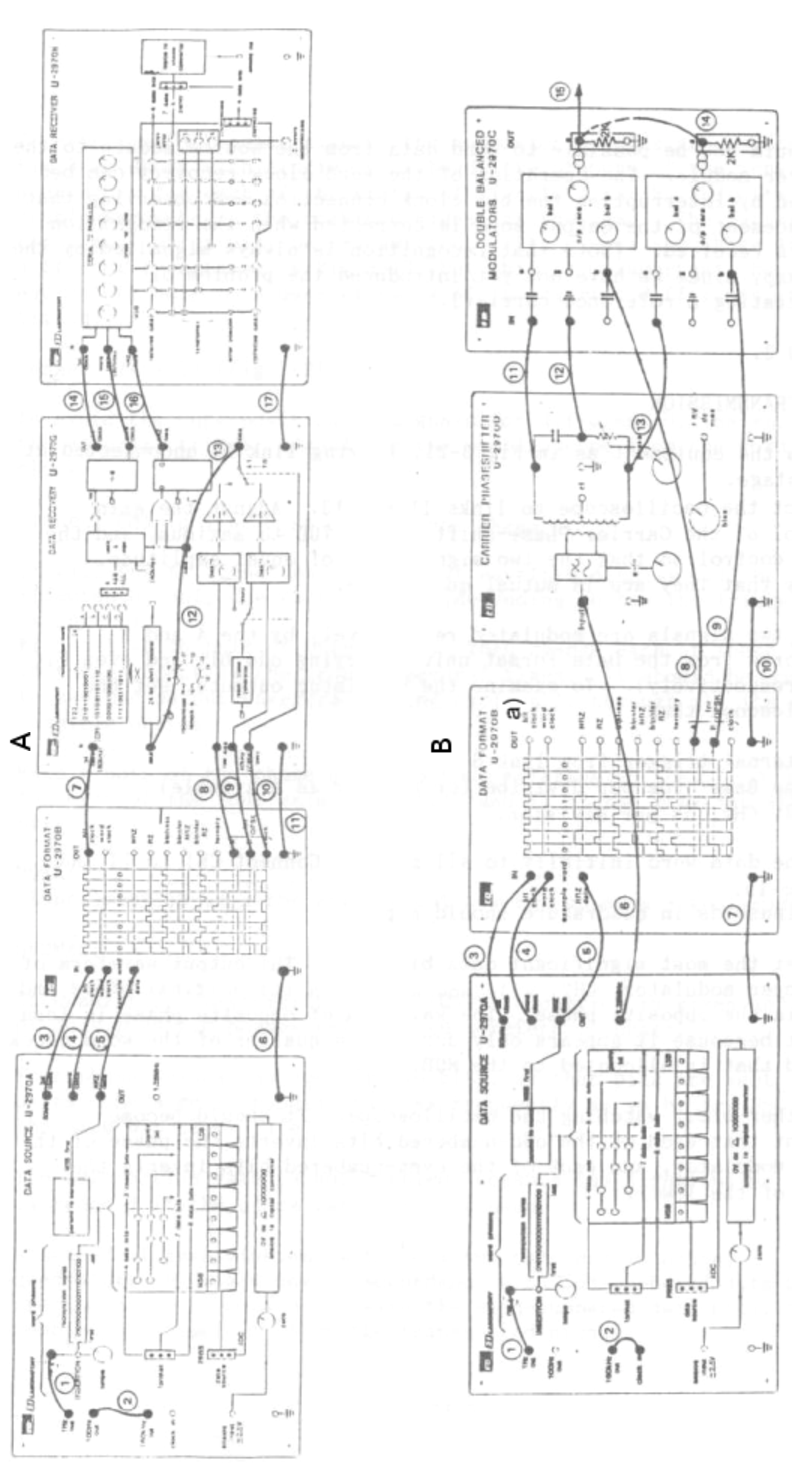
\includegraphics[scale=0.15]{montagem}
	\label{f_buck}
\end{figure}

